\scanpage{49}
% loc: cancelled continuation at head
\deleted{look at $V$ only (where $\overline V=V\unsure{\otimes|\ominus}_{\mathbb Q}\overline{\mathbb Q}$)}
\[
\deleted{\overline V^{G}\subset\overline V\cap g(\overline V)}
\]
\deleted{and to prove that it is an identity [for $\overline V^G\cap V=V^G$].}

% loc: first equivalence
Now the relation $x\in\overset{\deleted{\unsure{-}}}{V}\cap g(\overline V)$ is equivalent to :
\begingroup\makeatletter\tagsleft@true\makeatother
\[
x\in\overset{\deleted{-}}{V},\quad g^{-1}x\in\overline V \tag*{ds}
\]
\endgroup
% loc: locus and second equivalence
and obviously implies, if $\overline T$\inserted{$\subset\overline G$} is the \deleted{\unsure{declination|closure} of} \inserted{locus of} $g$ on $G_{\overline{\mathbb Q}}$
\[
x\in\overline V,\quad\deleted{\unsure{g^{-1}x}}\quad t\deleted{\unsure{^{-1}}}s^{-1}\in G_x(\mathbb C)\quad\text{for }t,s\in\overline T(\mathbb C),
\]
and is even equivalent to it.
% loc: stabilizer paragraph
In other words, if $G_x$ is the stabilizer of \deleted{$G$}$x$, which is an algebraic subgroup of $G$, \deleted{\unsure{one}} \inserted{the relation $x\in V\cap g(\overline W)$ is equi-}valent to :
\[
\deleted{\unsure{g}}\overline R\in\overline{G_x}\deleted{\unsure{(\mathbb C)}},
\]
where $\overline R$ is the closure of the image of $\overline T\times\overline T\longrightarrow\overline G$, $(s,t)\longmapsto s^{-1}t$.

% loc: image subgroup and equality question
Now let $\widehat R$ be the \unsure{image|image} of $\overline R$ in $G$, $H$ the subgroup it generates, $H\subset G$. \deleted{Thus the desired property is equivalent to which \unsure{?}} The relation ds is therefore equivalent to $\deleted{R}H\subset G_x$ i.e. $H$ fixes $x$.
% loc: left insertion at opening of proposition
\inserted{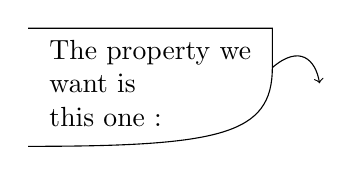
\begin{tikzpicture}[baseline=(n.base)]\node[align=left] (n) {The property we\\want is\\this one :};\draw (-1.55,0.7) -- (1.55,0.7) -- (1.55,0.2) .. controls (1.55,-0.65) and (0.9,-0.8) .. (-1.55,-0.8);\draw[->] (1.55,0.2) .. controls (1.9,0.5) and (2.1,0.3) .. (2.15,0);\end{tikzpicture}}
% loc: heavily cancelled proposition and replacement
For every $G$-module $V$, \deleted{and every $x\in V$, such that the stabilizer $G_x$ contains $R$, \inserted{i.e. such that $R$ fixes $x$,} one has that $x\in V^G$ i.e. $G_x=G$.}
\deleted{It suffices for this that the \illegible{1} be the subgroup generated by $R$, be equal to $G$. It is also necessary} that the invariants of $H$ and of $G$ (for every representation of $G$) be the same. It suffices that one have $H=G$, but this condition is not necessary a priori, for a Borel $k$-group of $G$ has this property.
% loc: NB at left of cancelled lines
\margin{NB $\deleted{\unsure{\overline T}}\overline R,\overline H$ do not depend on the choice of $g$ modulo $G(\overline{\mathbb Q})$, \deleted{\unsure{up to one|a priori}}}
% loc: sloping note above 5
% slanted
\margin{\uline{Look at} motives \uline{associated} with \uline{elliptic curves}}
% loc: item 5, first half
5) Of course, without even assuming that $k$ is algebraic over $\mathbb Q$, one can look at the functor (4.1). But it is no longer in general fully faithful, even if $k$ is of finite type over $\mathbb Q$, since for $\unsure{\mathcal M|M}$ a fixed \inserted{$\otimes$-category} of finite type $\subset\operatorname{Mot}(k)$, provided one enlarges $k$, one finds that \inserted{the} $T_{\mathrm{DR}}(M)$ \uline{contain} $T_{\mathrm B}(M)$, so the homomorphisms of mixed structures are simply the homomorphisms between the $T_{\mathrm B}(M)$ : idiotic !
% loc: closing lines of item 5
For fixed $M$, one can hope at the very best to have some disjointness result for $T_{\mathrm B}$ and $T_{\mathrm{DR}}$ if $k$ is $\pm$ moderate (for example to have estimates of minimum transcendence degree).
% No watermark lettering securely recoverable on this image; the reading supplied by C remains an audit question.
% archive sheet number: 48
